\documentclass[12pt, a4paper, onecolumn]{article}
\usepackage{graphicx}
\graphicspath{{plot/}}
\usepackage{fancyvrb}
\usepackage{topcapt}
%\usepackage{fancyref, marvosym, textcomp, layout, amsmath, amssymb}
\usepackage[textwidth={13.25cm}, vmargin={2.5cm}, nohead, includeheadfoot]{geometry}


\renewcommand{\contentsname}{目錄}
\renewcommand{\tablename}{表}
\renewcommand{\figurename}{圖}
%\renewcommand{\freffigname}{圖}
%\renewcommand{\freftabname}{表}
\title{統計分析結果的報導方式}
\author{Chen-Pan Liao}
%\date{2019/11/28}

\usepackage[
	%	pdfdirection={L2R},
	bookmarks=true,
	colorlinks=false,
	pageanchor=true,
	linktocpage=true,
	hyperfootnotes=true,
	breaklinks=true,
	%	pdflang={en-US},
	%	pdfprintscaling={none},
	pdfdisplaydoctitle=true,
	bookmarksopen=true,
	bookmarksopenlevel=2,
	unicode=true,
	xetex,
	bookmarksnumbered=true,
	pdfstartview={XYZ null null 1},
	pdfpagelayout={OneColumn},
	%	pdfpagelayout={TwoColumnRight},
	pdfpagemode={UseOutlines},
	%linkcolor=blue, citecolor=blue, filecolor=blue, urlcolor=blue,
	pdfborder={0 0 1},
	pdfauthor={Chen-Pan Liao},
	pdftitle={統計分析結果的報導方式},
	pdfsubject={統計學},
	% pdfcreator={LaTeX with pslatex},
	% pdfkeywords={statistics, R},
	% pdftrapped={Unknown},
	pdfinfo={License={CC BY-SA 4.0}}							
]{hyperref}

%% 西文字配置
\usepackage{amsmath}
%\usepackage{microtype}
\linespread{1.2}
\usepackage[no-math]{fontspec}
\setmainfont[Mapping=tex-text]{Latin Modern Roman}
\setsansfont[Mapping=tex-text]{Latin Modern Sans}
\setmonofont[Scale=MatchLowercase]{Sarasa Term CL Light}%
\usepackage{unicode-math}
\setmathfont{Latin Modern Math}

%% 中文字配置
\usepackage[
  CJKmath=true, 
  PunctStyle={quanjiao},
%  CheckSingle=true, 
  CJKglue = {\hskip0pt plus 3pt minus 0.5pt},
  CJKecglue = {\hskip3pt plus 8pt minus 0pt},
  Verb = false]
{xeCJK} 
\setCJKmainfont[Scale=0.97, BoldFont={Noto Serif CJK JP Bold}]{Noto Serif CJK JP}
\setCJKsansfont[Scale=0.97, BoldFont={}]{Sarasa Gothic CL}
\setCJKmonofont[Scale=MatchLowercase]{Sarasa Term CL Light} 
\newcommand{\nbs}{\hskip3pt plus 1pt minus 0pt}

%\usepackage[small, compact]{titlesec}
%\usepackage[marginal, perpage]{footmisc}


\begin{document}

\maketitle

\noindent
\includegraphics[width=1in]{cc.pdf}\\[2pt]
本文件全文之著作權屬廖鎮磐 (Chen-Pan Liao) 所有 (聲明日:\today),並採用姓名標示-相同方式分享 4.0 國際 (CC BY-SA 4.0;詳細內容請見 \url{http://creativecommons.org/licenses/by-sa/4.0/deed.zh_TW})。

\tableofcontents

\section{前言}
在進行統計分析之後,報導重要的統計結果並正確解讀結果才是負責任的方式。一般而言,在收隻樣本後必須報導描述性統計,包括中央趨勢 (如平均值或中位數) 、樣本數及變異程度 (如標準偏差或標準誤差);這些敘述性統計若內容太多可以改以圖或表的方式呈現。對於特別感到興趣的參數應計算其信賴區間。進行檢驗後應報導檢定統計量 (如$t$、$f$、$\chi^2$等) 、自由度與p-value,並報導合適的效果量 (如Cohan $d$、$r$、$R^2$等)。關於效果量在課堂中並未多加說明,且不同的效果量適合不同的統計方法,學生可按自己的能力決定是否報導效果量。

以下我將按不同的分析情況示範報導分析結果。我刻意報導較多細節而看來繁瑣,學生可以模仿我的內容以撰寫報告作業,但未來其它課程或學術報告時參考使用即可。最末一併附上計算及繪圖之R code。本文內容將隨課程進度持續增加內容。



\section{單樣本均值檢驗}
\subsection{常態情況}
檢驗 8.8, 10.3, 11.1, 7.7, 10.4, 10.5, 9.4, 9.5, 9.4, 9.1 之中央趨勢是否顯著不同於9。

結果指出,樣本平均$\pm$標準差為$9.62 \pm 0.987$ ($n = 10$)。由Shapiro-Wilk test檢驗常態性發現不能拒絕常態之虚無假設 ($W = 0.960$, $p = 0.790$),故以one-sample two-tailed Student-t test進行檢驗$H_0: \mu=9$。結果指出,平均值的95\%信賴區間為$\left[8.914, 10.236\right]$,無法拒絕$\mu = 9$的虚無假說 ($t = 1.986$, $\text{DF} = 9$, $p = 0.078$)。此外,Cohan $D = 0.627$顯示中度效果量。結論是,母體平均不顯著不等於9,但由中度效果量推測,不顯著可能是因樣本數不足造成的。

\subsection{非常態情況}
檢驗 2.5, 0.25, 0.01, 1.74, 0.39, 0.09, 0.82, 0.2, 0.84, 0.76 之中央趨勢是否顯著不同於2。

結果指出,樣本平均$\pm$標準差為$0.76 \pm 0.797$ ($n = 10$)。由Shapiro-Wilk test檢驗常態性發現拒絕常態之虚無假設 ($W = 0.841$, $p = 0.045$),故以Wilcoxon signed rank sum test進行檢驗$H_0: \text{中位數}=2$。結果指出,應拒絕中位數$=2$的虚無假說 ($\text{樣本中位數}=0.575$,$V = 2$, $p = 0.006$)。此外,多達90\% 的樣本小於2,顯示高度的效果量。結論是,母體中位數顯著不等於2且小於2。\footnote{在雙尾檢驗後若顯著可以藉樣本平均或中位數的大小直接解釋為顯著大於或小於。}

\section{配對兩樣本均值檢驗}
\subsection{常態情況}
檢驗以下配對樣本
\[
\begin{matrix}
x_1 & 8.8 & 10.3 & 11.1 & 7.7 &10.4 & 10.5 & 9.4 & 9.5 \\
x_2 & 9.2 & 10.4 & 11.6 & 7.7 & 10.6 & 11.6 & 11.4 & 10.4
\end{matrix}
\]
之差值 ($x_1 - x_2$) 中央趨勢是否顯著小於0.1。

結果指出,$x_1$與$x_2$之平均$\pm$標準差分別為$9.71 \pm 1.095$及$10.36 \pm 1.344$ ($n_\mathrm{pair} = 8$; 圖 \ref{fig:normal_paired_test}a)。差值平均$\pm$標準差為$-0.65\pm0.665$  (圖 \ref{fig:normal_paired_test}b)。由Shapiro-Wilk test檢驗差值之常態性發現不能拒絕常態之虚無假設 ($W = 0.883$, $p = 0.202$),故以two-sample paired t-test檢驗$H_0: \mu_1 - \mu_2 \geq 0.1$。結果指出,應拒絕虚無假設 ($t = -3.188$, $\text{DF} = 7$, $p = 0.015$)。此外,差值平均之95\%信賴區間為$\left[-1.206, -0.0936\right]$,且Cohan $D = 1.728$顯示高度效果量。結論是:差值平均顯著小於0且差距之效果量甚高。

\begin{figure}[ht!]
	\centering
	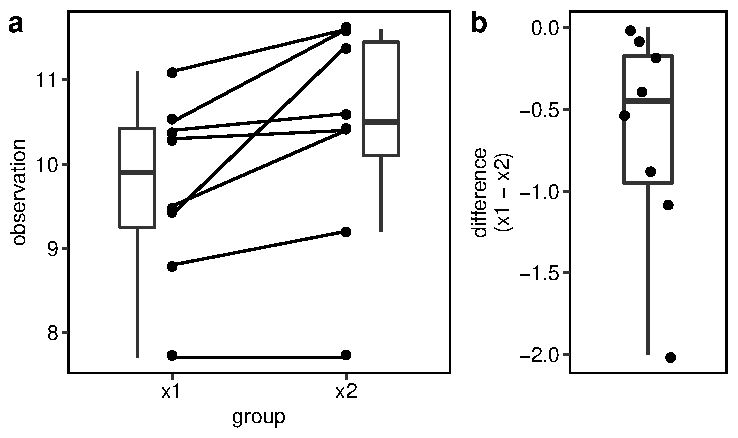
\includegraphics[]{normal_paired_test.pdf}
	\caption{配對兩樣本的觀測值盒形圖 (a) 及差值盒形圖 (b)。}
	\label{fig:normal_paired_test}
\end{figure}

\subsection{非常態情況}
檢驗以下配對樣本
\[
\begin{matrix}
x_1 & 5.1 & 6.9 & 7.2 & 6.5 & 7.2 & 6.4 & 5.3 & 7.7 \\
x_2 & 5.6 & 6.2 & 6.6 & 6.7 & 6.7 & 5.8 & 4.8 & 8.1
\end{matrix}
\]
之差值 ($x_1 - x_2$) 中央趨勢是否顯著偏離1。

結果指出,$x_1$與$x_2$之平均$\pm$標準差分別為$6.538 \pm 0.924$及$6.313 \pm 0.975$ ($n_\mathrm{pair} = 8$;圖 \ref{fig:non-normal_paired_test}a)。差值平均$\pm$標準差為$0.225\pm0.501$ (圖 \ref{fig:non-normal_paired_test}b)。由Shapiro-Wilk test檢驗差值之常態性,結果顯示應拒絕常態之虚無假設 ($W = 0.797$, $p = 0.026$),故以Wilcoxon signed rank sum test進行檢驗$H_0: \text{差值中位數}=1$。結果顯示,差值中位數顯著不等於1 ($V = 0$, $p = 0.014$) 而是小於1。此外,100\% 的樣本差值小於1,具極高的效果量。結論是,差值母體中位數顯著小於1且效果量高。

\begin{figure}[ht!]
	\centering
	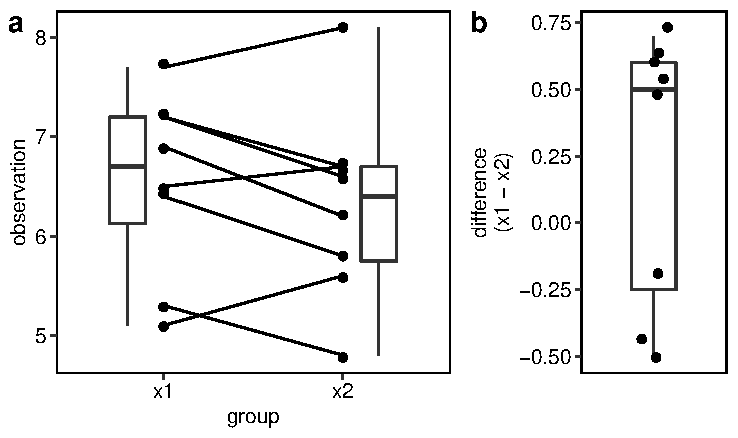
\includegraphics[]{non-normal_paired_test.pdf}
	\caption{配對兩樣本的觀測值盒形圖 (a) 及差值盒形圖 (b)。}
	\label{fig:non-normal_paired_test}
\end{figure}

\section{獨立兩樣本均值檢驗}
\subsection{常態情況}
檢驗以下兩獨立樣本
\[
\begin{matrix}
x_1 & 8.6 & 10 & 9.2 & 10.2 & 11.4 & 10.7 & \\
x_2 & 9.7 & 8.8 & 9.2 & 10.2 & 9.3 & 7.6 & 8.6
\end{matrix}
\]
之中央趨勢是否顯著偏離0。

結果指出,$x_1$與$x_2$之平均$\pm$標準差分別為$10.02 \pm 1.095$及$9.057 \pm 0.836$ ($n_1 = 6$,$n_2 = 7$;圖 \ref{fig:normal_independent_test})。由Shapiro-Wilk test檢驗差值之常態性發現二樣本皆不能拒絕常態之虚無假設 ($x_1$,$W = 0.985$, $p = 0.975$;$x_2$,$W = 0.976$, $p = 0.938$),故以Welch two-Sample t-test檢驗$H_0: \mu_1 - \mu_2 = 0$。結果指出不應拒絕虚無假設 ($t = 1.848$, $\text{DF} = 9.794$, $p = 0.095$)。此外,差值平均之95\%信賴區間為$\left[-0.201, 2.120\right]$,且Cohan $D = 1.044$顯示高度效果量。結論是二樣本平均無顯著差異,但效果量甚高,可能因樣本數不足而發生型二錯誤。

\begin{figure}[ht!]
	\centering
	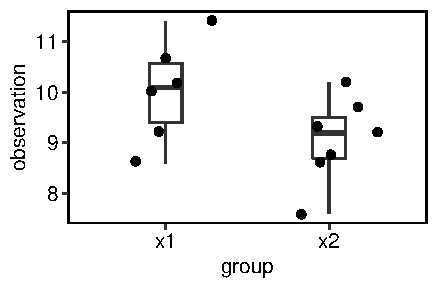
\includegraphics[]{normal_independent_test.pdf}
	\caption{獨立兩樣本的觀測值盒形圖。}
	\label{fig:normal_independent_test}
\end{figure}

\subsection{非常態情況}
檢驗以下兩獨立樣本
\[
\begin{matrix}
x_1 & 0 & 0.1 & 0.7 & 0.7 & 0.9 & 0.7 & 0 & 0.9 \\
x_2 & 0.7 & 1.6 & 0.6 & 0.4 & 1.7 & 0.2 & 1.4 & 
\end{matrix}
\]
之中央趨勢是否顯著偏離0。

結果指出,$x_1$與$x_2$之平均$\pm$標準差分別為$0.5 \pm 0.396$及$0.943 \pm 0.611$ ($n_1 = 8$;$n_2=7$;圖 \ref{fig:non-normal_independent_test})。由Shapiro-Wilk test檢驗差值之常態性發現$x_1$拒絕常態之虚無假設 ($x_1$,$W = 0.794$, $p = 0.024$;$x_2$,$W = 0.890$, $p = 0.276$),故以Mann-Whitney U test檢驗$H_0: \text{Median}_1 - \text{Median}_2 = 0$。結果指出不應拒絕虚無假設 ($W = 18.5$, $p = 0.292$)。此外,Cliff's $d=0.339$顯示中等程度效果量。結論是,二樣本之中位數無顯著差異,但效果量程中度,可能因樣本數不足而發生型二錯誤。
\begin{figure}[ht!]
	\centering
	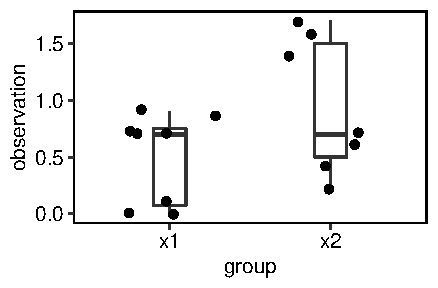
\includegraphics[]{non-normal_independent_test.pdf}
	\caption{獨立兩樣本的觀測值盒形圖。}
	\label{fig:non-normal_independent_test}
\end{figure}

\section{多樣本單因子均值檢驗}
\subsection{常態且變方同質情況}
檢驗以下三獨立樣本
\[
\begin{matrix}
x_1 & 5.16 & 4.24 & 4.7 & 4.58 & 6.06 & 5.99 &  \\
x_2 & 4.91 & 5.65 & 5.58 & 5.12 & 4.32 & & \\
x_3 & 7.65 & 6.64 & 7 & 5.57 & 5.84 & 8.48 & 7.07
\end{matrix}
\]
之中央趨勢是否相等。

三樣本的描述性統計如表 \ref{table:oneway_ANOVA}。由於三組樣本分布並不顯著偏離常態 (Shapiro-Wilk test,$p_1 = 0.709$,$p_2 = 0.85$,$p_3 = 0.925$),且變異數不顯著不等 (Bartlett test,$\chi^2 = 0.469$, $\text{DF} = 2$,$p = 0.791$),故以one-way ANOVA檢驗$H_0:\mu_1 = \mu_2 = \mu_3$。結果顯示,$x$為顯著因子 ($f = 9.297$,$\text{DF} = (2, 15)$, $p = 0.0024$),且$\eta^2$顯示有55.3\% 的變異量可由$x$因子解釋。接下來以Tukey's range test進行多重比較,結果顯示,$x_1$與$x_3$存在顯著差異,而$x_2$與另二組皆無顯著差異 (表 \ref{table:oneway_ANOVA_post};圖 \ref{fig:oneway_ANOVA})。

\begin{table}[ht!]
	\topcaption{獨立三樣本的描述性統計。} 
	\centering
	\begin{tabular}{lrrr}
		\hline
		Group & Mean & SD & $n$\\ 
		\hline
		$x_1$ & 4.94 & 0.77 &   6 \\ 
		$x_2$ & 5.86 & 0.79 &   5 \\ 
		$x_3$ & 6.65 & 0.59 &   7 \\ 
		\hline
	\end{tabular}
	\label{table:oneway_ANOVA}
\end{table}

\begin{table}[ht!]
	\topcaption{獨立三樣本的事後多重比較。} 
	\centering
	\begin{tabular}{lrrrr}
		\hline
		Comparison & Estimate & 95\% CI lower & 95\% CI upper & $p_{\mathrm{adj}}$ \\ 
		\hline
		$x_2-x_1$ & 0.917 & $-0.200$ & 2.034 & 0.117 \\ 
		$x_3-x_1$ & 1.704 & 0.677 & 2.730 & 0.002 \\ 
		$x_3-x_2$ & 0.787 & $-0.293$ & 1.867 & 0.175 \\ 
		\hline
	\end{tabular}
	\label{table:oneway_ANOVA_post}
\end{table}

\begin{figure}[ht!]
	\centering
	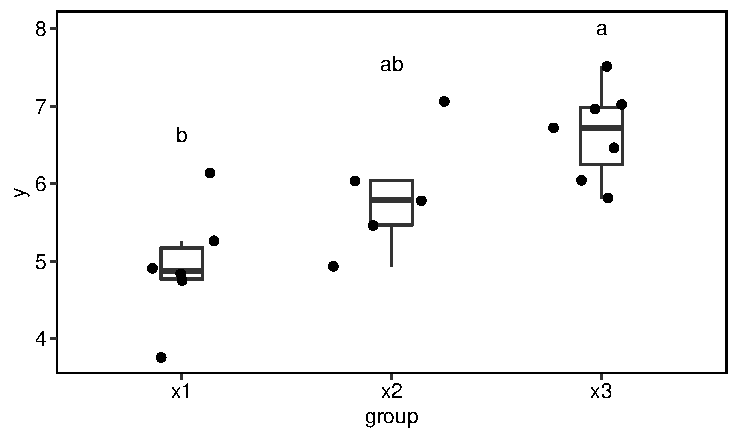
\includegraphics[]{oneway_ANOVA.pdf}
	\caption{獨立三樣本的觀測值盒形圖。上方字母為多重比較的分群結果;若任二組存在相同字母則表示不存在顯著差異,反則反之。}
	\label{fig:oneway_ANOVA}
\end{figure}

\subsection{常態且變方異質情況}
檢驗以下三獨立樣本
\[
\begin{matrix}
x_1 & 3.18 & 4.12 & 3.52 & 3.29 & 5.13 & 5.2 &  \\
x_2 & 5.7 & 5.21 & 7.62 & 8.19 & 6.26 & & \\
x_3 & 7.12 & 7.4 & 8.19 & 3.66 & 3.78 & 11.9 & 6.87
\end{matrix}
\]
之中央趨勢是否相等。

三樣本的描述性統計如表 \ref{table:Welch_ANOVA}。由於三組樣本分布並不顯著偏離常態 (Shapiro-Wilk test,$p_1 = 0.158$,$p_2 = 0.593$,$p_3 = 0.388$),且變異數顯著不相等 (Bartlett test,$\chi^2 = 6.340$, $\text{DF} = 2$,$p = 0.042$),故以Welch one-way ANOVA檢驗$H_0:\mu_1 = \mu_2 = \mu_3$。結果顯示,$x$為顯著因子 ($f = 8.248$,$\text{DF} = (2, 8.953)$, $p = 0.009$),且$\eta^2$顯示有34.77\% 的變異量可由$x$因子解釋。接下來以Games-Howell method進行多重比較,結果顯示,$x_1$與$x_3$存在顯著差異,而$x_2$與另二組皆無顯著差異 (表 \ref{table:Welch_ANOVA_post};圖 \ref{fig:Welch_ANOVA})。

\begin{table}[ht!]
	\topcaption{獨立三樣本的描述性統計。} 
	\centering
	\begin{tabular}{lrrr}
		\hline
		Group & Mean & SD & $n$ \\ 
		\hline
		$x_1$ & 4.073 & 0.906 &    6 \\ 
		$x_2$ & 6.596 & 1.267 &    5 \\ 
		$x_3$ & 6.989 & 2.803 &    7 \\ 
		\hline
	\end{tabular}
	\label{table:Welch_ANOVA}
\end{table}

\begin{table}[ht!]
	\topcaption{獨立三樣本的事後多重比較。} 
	\centering
	\begin{tabular}{lrrrrr}
		\hline
		Comparison & Estimate & 95\% CI & $t$ & DF & $p_{\mathrm{adj}}$ \\ 
		\hline
		$x_2-x_1$ & 2.523 & $\left[0.536 , 4.509\right]$ & 3.727 & 7.103 & 0.017 \\ 
		$x_3-x_1$ & 2.915 & $\left[-0.345 , 6.175\right]$ & 2.598 & 7.420 & 0.077 \\ 
		$x_3-x_2$ & 0.393 & $\left[-2.973 , 3.758\right]$ & 0.327 & 8.840 & 0.943 \\ 
		\hline
	\end{tabular}
	\label{table:Welch_ANOVA_post}
\end{table}

\begin{figure}[ht!]
	\centering
	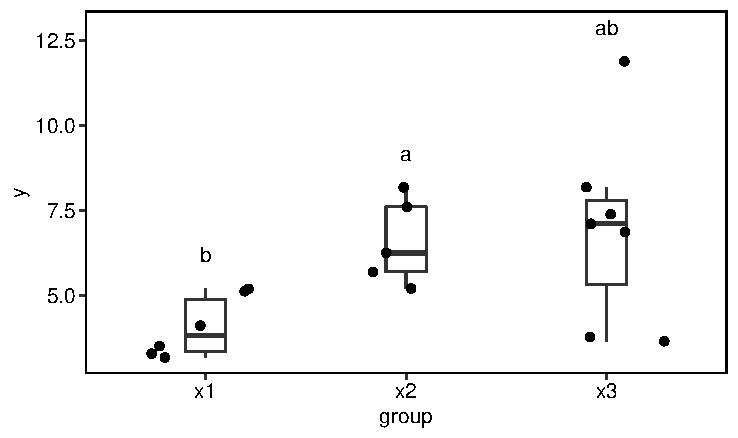
\includegraphics[]{Welch_ANOVA.pdf}
	\caption{獨立三樣本的觀測值盒形圖。上方字母為多重比較的分群結果;若任二組存在相同字母則表示不存在顯著差異,反則反之。}
	\label{fig:Welch_ANOVA}
\end{figure}

\subsection{非常態情況}
(待撰)

\section{多樣本雙因子均值檢驗}
(待撰)

\section{簡單線性迴歸}
以下樣本
\[
\begin{matrix}
x & 8.8 & 10.3 & 11.1 & 7.7 & 10.4 & 10.5 & 9.4 & 9.5\\
y & 17 & 19.7 & 21.7 & 14.4 & 20 & 21.1 & 19.8 & 18.9
\end{matrix}
\]
中,$y$為應變數,$x$為自變數,建立$y = \beta_0 + \beta_1 x + \varepsilon$的簡單線性迴歸。

簡單線性迴歸之結果如表 \ref{table:simple_regression} 及圖 \ref{fig:simple_regression}a。結果顯示,每$x$增加1單位使$y$平均顯著增加2.069單位,應拒絕$H_0: \beta_1 = 0$ (表 \ref{table:simple_regression}a)。就效果量而言,自變數可解釋$R^2 = 92.4\%$之變異量,屬高效果量。就迴歸診斷而言,殘差之Q-Q圖 (圖 \ref{fig:simple_regression}b) 顯示殘差呈輕微右偏態,Shapiro-Wilk test顯示殘差並未顯著偏離常態分布 ($W = 0.848$,$p=0.090$),模型配適尚可。結論是,自變數顯著地增加應變數且效果明顯。

\begin{table}[ht!]
	\topcaption{簡單線性迴歸之結果。} 
	\centering
	\small
	\begin{tabular}{rrrrr}
		\hline
		Variable & Estimate $\pm$ Std.~Error & $t$ (DF = 6) & $p$ & 95\% CI \\ 
		\hline
		Intercept & $-1.016\pm2.408$ & $-0.422$ & 0.688 & $\left[-6.909, 4.877\right]$ \\ 
		$x$ & $2.069\pm0.247$ & 8.389 & $<0.001$ & $\left[1.465, 2.672\right]$ \\ 
		\hline
	\end{tabular}
	\label{table:simple_regression}
\end{table}

\begin{figure}[ht!]
	\centering
	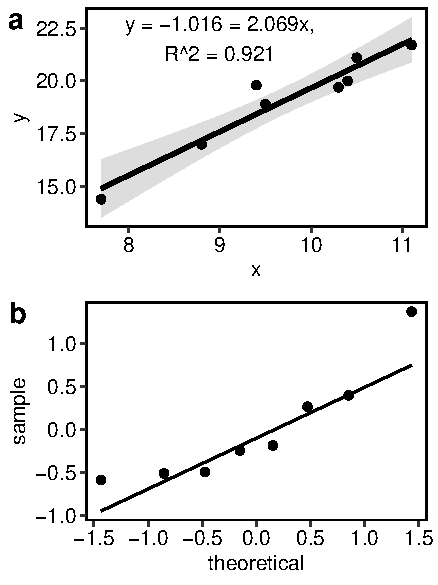
\includegraphics[]{simple_regression.pdf}
	\caption{簡單線性迴歸之散布圖及迴歸線 (a) 及Q-Q plot (b)。圖中灰色區域為 95\% confidence pointwise band。}
	\label{fig:simple_regression}
\end{figure}


\section{簡單相關}
\subsection{雙常態分布情況}
以下樣本
\[
\begin{matrix}
x_1 & 8.8 & 10.3 & 11.1 & 7.7 & 10.4 & 10.5 & 9.4 & 9.5\\
x_2 & 17 & 19.7 & 21.7 & 14.4 & 20 & 21.1 & 19.8 & 18.9
\end{matrix}
\]
中,分析二變數之間的相關性。

首先以Shapiro-Wilk multivariate normality test檢驗$x_1$與$x_2$是否偏離雙變量常態分布,結果顯示不能拒絕$H_0: x_1與x_2之母體聯合分配為常態$ ($W = 0.860$,$p = 0.120$),故可計算Pearson correlation。結果指出,$r = 0.960$屬高度正相關且應拒絕$H_0:\rho=0$ (95\% CI = $\left[ 0.789, 0.993\right]$, $t = 8.389$,$\text{DF} = 6$,$p < 0.001$;圖 \ref{fig:simple_cor})。結論是,$x_1$與$x_2$間存在顯著的高度正向線性相關性。

\begin{figure}[ht!]
	\centering
	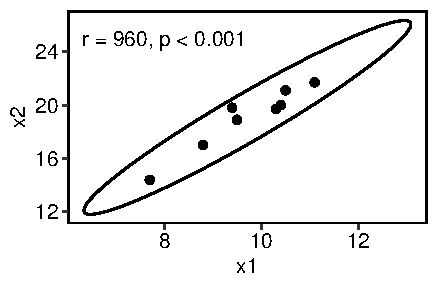
\includegraphics[]{simple_cor.pdf}
	\caption{$x_1$與$x_2$散布圖。圖中楕圓區域表示相關性之95\% confidence ellipse。}
	\label{fig:simple_cor}
\end{figure}

\subsection{次序相關}
以下樣本
\[
\begin{matrix}
x_1 & 7.5 & 5.4 & 5.9 & 6.1 & 7.9 & 7.9 & 6.6 & 6\\
x_2 & 0.3 & 0.2 & 4.4 & 2.7 & 0.1 & 1 & 0.3 & 0.5
\end{matrix}
\]
中,分析二變數之間的相關性。

首先以Shapiro-Wilk multivariate normality test檢驗$x_1$與$x_2$是否偏離雙變量常態分布,結果顯示不能拒絕$H_0: x_1與x_2之母體聯合分配為常態$ ($W = 0.739$,$p = 0.006$),故計算Spearman's rank correlation coefficient。結果指出,$r_\mathrm{s} = -0.241$屬低度負相關且無法拒絕$H_0:\rho_\mathrm{s}=0$ ($S = 104.24$,$p=0.565$;圖 \ref{fig:spearman_cor})。結論是,$x_1$與$x_2$間不存在顯著次序相關性。

\begin{figure}[ht!]
	\centering
	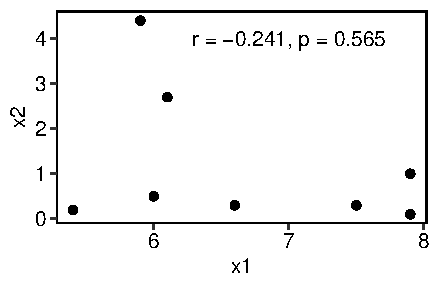
\includegraphics[]{spearman_cor.pdf}
	\caption{$x_1$與$x_2$散布圖。}
	\label{fig:spearman_cor}
\end{figure}

\section{卡方適合度檢驗}
(待撰)

\section{卡方獨立性檢驗}
(待撰)

\clearpage
\onecolumn
\appendix
\section{R code}
以下為本文中所有產生資料、進行分析、製作表格與繪圖之R code。
\VerbatimInput[fontsize=\normalsize, baselinestretch=0.769, formatcom=\xeCJKVerbAddon, numbers=left, numbersep=2mm, framesep=3mm, frame=leftline]{plot/report-results.R}

\end{document}
